% !TEX root = ../rapport.tex

\section{Software}
Nu er bilen optimeret mest muligt rent hardwaremæssigt. For at kunne kører den hurtigst muligt omgangstid skal der også udvikles noget sofware. Softwaren skal henholdsvis bruges til at:
\begin{itemize}
\item Kommunikere med bluetooth.
\item Kommunikere med sensorer.
\item Aflæsning af optisk dekoder og stregdetektor.
\item Lave et map af den ukendte bane.
\item Styre motoren i forhold til det gemte map.
\end{itemize}
Alt software til bilen er udviklet i assembly.


% !TEX root = ../rapport.tex
\section{Bootloader}
Programmerstikket til mikroprocessoren er ikke nem at tilgå, når bilen er fuldt monteret. For at kunne iterere hurtigt og undgå at skulle skille bilen ad og samle bilen hele tiden, blev der udviklet en bootloader.

\subsection{Bluetooth}
For at sikre, der kan skabes kontakt med bootloaderen, styrer bootloaderen bluetoothkommunikationen.
\subsubsection{Baudrate}
En række stresstests blev udført for at finde den hurtigste, stabile baudrate mellem mikrocontrollerens og bluetoothmodulet. Dataflowet er primært fra mikrocontrollerens til pc. Stresstestene er opbygget derefter.
En enkelt byte med værdien, x, sendes til mikrocontrollerens, hvorefter mikrocontrollerens sender x kb tilbage.
Se ``avr/src/bt/tests/replykb.asm''.
Forskellige baudrates blev stresstestet ved 250 kB. Den højeste af disse, der ikke havde datatab, var 38 kbps. Disse tests blev udført uden parity bit, med én stop bit og med 8 databits. Det er også denne opsætning der antages fremadrettet. Se eventuelt ``avr/src/bt/bt\_setup.asm''. Det vil sige 9 bits i alt per overført byte. Det giver en teoretisk overførselshastighed på $38 kbps / 9 bpB \simeq 4.2 kB/s$ Der kunne have været eksperimenteret med parity bits og flere stopbits ved højere baudrates, men der var ikke umiddelbart behov for hurtigere overførselshastigheder.
\subsubsection{Output Buffer}
Med en clockfrekvens på 16 MHz går der $16*10^6 / 4.2*10^3 \simeq 3810$ cycles mellem, der kan sende bytes. Hvis man ønsker at sende $x$ bytes synkront, skal programmet i alt vente $(x-1)*3810$ cycles. For at udnytte disse cycles i stedet for at vente, implementeres en buffer i sram.
Se ``avr/src/bt/bt\_tr.asm''.
Bufferen består af en byte liste med en fast længde allokeret i sram samt to pointers, der også er allokeret i sram. Listen indeholder de bytes, der ønskes sendt, samt den frie plads i bufferen. Bytes i det frie område kan være bytes, der allerede er sendt, eller bytes, der endnu ikke er blevet skrevet over siden mikrocontrollerens sidste reset. En store pointer peger på den byte i listen, der blev tilføjet sidst. En send pointer peger på den byte i listen, der blev sendt sidst.
I initialiseringen af bufferen sættes de to pointere til at pege på den samme byte i listen.
Når der ønskes en byte sendt, inkrementeres store pointeren, og byten skrives til den adresse i listen store pointeren repræsenterer. Interrupt enableren for når UART data registeret er tomt sættes højt, så bufferen bliver informeret, når der kan sendes en byte.
Når der kan sendes en byte, og der er bytes i bufferen, der endnu ikke er sendt (store pointeren og send pointeren har ikke samme værdi), inkrementeres send pointeren, og den byte, send pointeren peger på sendes.

Hvis en af pointerne, efter at blive inkrementeret, peger på byten lige efter listens sidste byte, sættes pointeren til den første byte i listen.
Hvis store pointeren, efter at blive inkrementeret og eventuelt rykket til den første byte i listen, peger på samme adresse som send pointeren, er der overflow i bufferen. Det håndteres på nuværende tidspunkt ikke.
TODO: Der skal et billede ind her

\subsection{Protokol}
Bootloaderen styrer bluetoothkommunikationen og indeholder en overordnet kommunikationsprotokol.
Den første byte, initial byte, bootloaderen modtager, afgør, hvordan bootloaderen skal håndtere de næstkommende bytes.
85: Set. 85 gemmes som den første byte i inputbufferen. De to næstkommende bytes gemmes også, før der hoppes til kommando interruptet. Herefter forventer bootloaderen en ny initial byte.
87: Ping. Bootloaderen sender 87 tilbage med det samme. Herefter forventer bootloaderen en ny initial byte.

For at undgå at skulle opdatere bootloaderen, hvis der blev implementeret andre kommandoer i applikationsprotokollen, blev der implementeret en variabel kommando med initial byte: 86.
Den næstkommende byte beskriver længden, n, af kommandoen. De derefter næstkommende, n, bytes gemmes i inputbufferen, før der hoppes til kommando interruptet.
Bemærk:
[85, X, X] og [86, 3, 85, X, X] er ekvivalente.
[87] er ping kommandoen til bootloaderen. [86, 1, 87] er en kommando [87] til applikationen.

Længden er kun variabel for bootloaderen. Der gives ingen information til applikationen om længden af kommandoen.

Når der er en hel kommando (liste af bytes) klar til applikationen, hoppes til 0x2A, en udvidelse af interrupt vektor tabellen.

% !TEX root = ../rapport.tex
\newpage
\subsection{I2C kommunikation}
Til at kommunikere med de digitale komponenter, herunder vores udleveret accelerometer og gyroskop, anvendes den kommunikationsprotokol kaldet I2C eller TWI (”two-wire interface”). Navnet ”two-wire interface” kommer af, at hele kommunikationen foregår over kun 2 ledninger, men hvor der samtidig er mulighed for at kommunikere med mange komponenter.

\begin{figure}[ht]
    \centering
    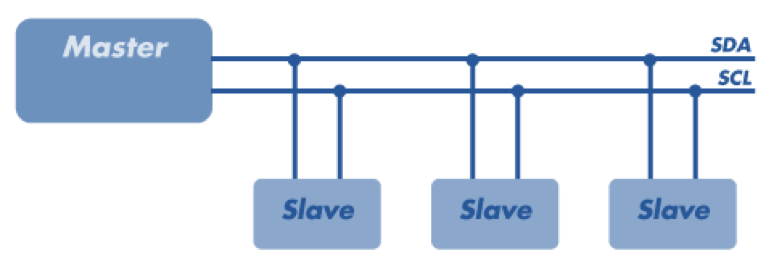
\includegraphics[width=0.8\textwidth]{kapitler/billeder/i2c-princip.png}
    \caption{Viser en skitse af hvordan opsætningen kan laves mellem
én ”master” og flere ”slaver”, kun ved brug af to forbindelser.}
    \label{fig:i2cprincip}
\end{figure}

De to forbindelser der bruges til vores TWI kommunikation hedder SCL (”Serial Clock Line”) og SDA (”Serial Data Line”). SCL er en clock der sættes af master, for at både master og slaven snakker og lytter ved en fælles frekvens. SDA er den forbindelse, hvor alt data bliver overført både fra slaven til master, men også fra master til slaven. Denne form for kommunikation kaldes for halv-duplex, og fungere ligesom en walkie talkie, hvor der kun er én der snakker af gangen, imens den anden lytter.

\subsubsection{Kommunikationsprotokol}

Kommunikationen mellem master og slave, foregår ud fra en bestemt protokol, som er opgivet ved den enkelte slaves datablad. Denne protokol er den samme for accelerometeret og gyroskopet, og er illustreret på figur \ref{fig:i2conebyte}. 

\begin{figure}[ht]
    \centering
    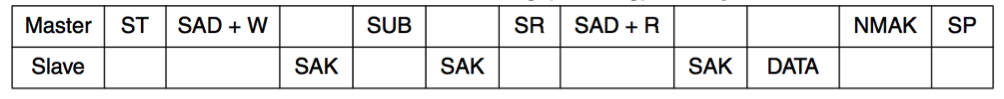
\includegraphics[width=1\textwidth]{kapitler/billeder/i2c-onebyte.png}
    \caption{Kommunikationsprotokol for gyroskopet via I2C}
    \label{fig:i2conebyte}
\end{figure}

Figur \ref{fig:i2conebyte} viser skridt for skridt, hvordan kommunikationsprotokollen er opbygget, hvis man vil læse data én gang fra én af vores to digital komponenter.

Protokollen indeholder følgende instruktioner for at modtage én data byte:

\begin{enumerate}
\item ST (”Start Bit”): Master sender et start bit til alle slaverne, for at starte kommunikationen.
\item SAD+W (”Slave Adress + Write”): Master sender en slave adresse på 7 bits, og det sidste bit beskriver om der skal læses eller skrives, i dette tilfælde skal der skrives. Adressen er specifik for hver komponent og fortæller hvilken slave, som resten af kommunikationen kommer til at foregå med. Det sidste bit indikere, at masteren vil skrive noget til slaven.
\item SAK (”Slave Acknowledge”): Slaven med den valgte adresse sender er ACK bit tilbage, som fortæller at den har hørt hvad masteren sagde, og gør klar til at læse næste instruktions.
\item SUB (”Sub adress”): Master sender herefter en underadresse. Denne underadresse er en 7 bit adresse, som fortæller hvilken register inde i den valgte komponent, der gerne vil adresseres.
\item SAK (”Slave Acknowledge”): Slaven sender endnu et SAK bit, og gør klar til næste instruktion.
\item SR (”Repeated Start”): Master sender herefter et gentagende start bit. Der skal altid sendes en start/repeated start instruktion, hver gang der skiftes mellem at læse eller skrive. Ved repeated start vedholdes forbindelsen til slaven, og slaven ved derfor allerede hvilken underadresse, der herefter skal læses fra.
\item SAD+R (”Slave Adresse + Read”): Master sender herefter igen slave adressen, samt én read bit, for at ændre at vi nu gerne vil læse på slaven, modsat at vores tidligere write, som skrev til slaven.
\item SAK (”Slave Acknowledge”):  Slaven sender en ACK bit.
\item DATA (”Data Byte”): Slaven sender efterfølgende en data byte til master.
\item NMAK (”Master Not Acknowledge”): Herefter sendes én NMAK fra master til slaven, for at indikere at der ikke skal læses mere data.
\item SP (”Stop Bit”): Til sidst sender master et stop bit, for at afslutte kommunikationen.
\end{enumerate}

% !TEX root = ../rapport.tex
\newpage
\section{Lap timer}
Formålet med Lap timeren er at have et stykke kode som måler og returnere omgangstiden, for hver omgang bilen køre. Lap timeren er baseret på "timer1" og er derfor den største timer. Lap timeren bliver udover omgangstid, også brugt af andre kode moduler, til at tage tid.
\subsection{Opsætning af Lap timer}
\subsection{Kode}
\subsection{Macro's}

* Valg af prescaler (udregninger)\\
	-præcision
	-maks/min omgangs tider 
	
* 24-bit register\\
% !TEX root = ../rapport.tex
\newpage

\section{Motor omdrejninger (kode)}

% !TEX root = ../rapport.tex
\newpage
\section{Kortlægning af bane}
Den bedste omgangstid afhænger af mange elektriske komponenter, som bindes sammen af software.
Denne software skal ud fra disse analoge og digital komponenter kunne analysere banen, og ud fra dette
kortlægge banen. Byggestenen til opbygning af denne kortlægning, kan ses på figur \ref{fig:mapflow}.

\begin{wrapfigure}{r}{0.35\textwidth}
  \vspace{-10pt}
  \begin{center}
      \includegraphics[width=0.25\textwidth]{kapitler/billeder/mapflow.png}
    \end{center}
    \vspace{-10pt}
    \caption{Viser grundstenene af koden til kortlægning af banen.}
    \label{fig:mapflow}
\end{wrapfigure}

Som der ses på figur \ref{fig:mapflow}, er pincippet bygget meget simpelt op, og kan beskrives ved følgende punkter:

\begin{itemize}
\item Venter på interrupt fra hvid-streg sensor (Tiltøj til flowchart)
\item Når den hvide streg er registeret, gemmen den omdrejningstælleren.
\item Herefter køres et loop, som bruger gyroskopet til at tjekke om der drejes.
\item Hvis vi drejer, gemmes omdrejningstæller og længden af det lige stykke regnes.
\item Status for et lige stykke, samt længden af stykket gemmes i SRAM.
\item Nyt loop tjekker om svinget er slut. Hvis sving er slut, gemmes omdrejnignstæller.
\item Status for sving, samt længde af sving gemmes i SRAM, og koden starter forfra.
\item Ved næste hvid-streg interrupt stoppes kortlægningen.
\end{itemize}

Når koden er færdig, vil alle sving og lige stykker være defineret i SRAM og koden vil blive behandlet
af et seperat program. 

% !TEX root = ../rapport.tex
\newpage

\subsection{kortlæsning}

Kodemodulet "Kortlæsnings modulet" benytter et map over banen, til at køre efter. Kortlægning kan der læses mere om i afsnit \textbf{kortlægning}.\\

\begin{figure}[ht]
\centering
\includegraphics[width=0.4\textwidth]{kapitler/billeder/mread/mread_ov.png}
\caption{Overordnet flowchart over map read koden}
\label{fig:mread}
\end{figure}

Inden bilen kan køre efter kortet, er det vigtigt at bilen kender sin position på banen. Kodemodulet starter derfor med at finde målstregen, ved brug af streg sensoren. Dernæst indlæses det kommende bane segment. Hvert segment har et status register, som fortæller om det er et sving eller lige stykke. Ud over status registrer, er der også to 8-bit registre som indeholder længden af det pågældende segment. Programmet bruger informationen til at vælge imellem 2 rutiner, rutinen for sving eller rutinen for lige strækninger. Når en af de følgende rutiner er blevet udført og bilen passeret bane segmentet, loades på ny et nyt banesegment.\\
\\
Når rutinen for sving kaldes, tændes elektromagneten for at forbedre grebet. Bilens hastighed bliver sat til den maksimale hastighed for sving.\\
\\
Når rutinen for lige segment kalde, slukkes elektromagneten og hastighed for bilen siddes til max. Ud over det, tjekkes der om næste segment er lige eller et sving. Hvis næste segment er lige, bibeholdes den maksimale hastighed. Hvis næste segment derimod er et sving, beregnes hvornår nedbremsningen skal finde sted, for at nå ned på den maksimale hastighed for sving. Beregningerne for hvornår der skal bremses, sker ved ved at den ønskede bremselængden trækkes fra segmentets længde. Bremselængden er en konstant distance som kan ændres i programmet. Til nedbremsningen benyttes elektromagneten for at skabe mere friktion, samt H-broen til at vende strømmen på motoren.\\



\subsection{Delkonklusion}
Skriv en del konklusion her..